\section{Overall design}
\subsection{PIN codes}
The user will have to enter a PIN code on the terminal numpad to verify ownership of the petrol card to the terminal. The terminal will send the PIN signed by its private key with the plain text of the PIN to the smartcard through the secure channel. By which the smartcard will reply with whether the PIN number is correct or not.

\subsection{Cryptography}
A certificate consisting of a public and private key will be first created on the back-end (the overall system acting as the Certificate Authority). Whenever a new smartcard is personalized, it will store the certificate of the CA, create public and private key for itself and a timestamp of the last update of certificate revocation list which is signed by the CA certificate. Each terminal will have the same setup: CA certificate, its own public and private key, and signed timestamp of the last updated certificate revocation list.

\subsection{CA certificate stored in Terminals/Smartcards}
The main certificate from the CA stored in each terminal and smartcard is used to verify the validity and authenticity of each certificate during communication. Each end point, i.e both smartcard and terminal alike, will verify the certificate of the other end point it is connecting to, whether the certificate has been revoked or not by the CA. This way when the CA has been notified of abuse or breach in one of the end points, it will only take 24 hours for each end point to know of the revocation of a particular certificate.

\subsection{Public and Private keys in Terminals/Smartcards}
Public and private keys in each end point will be used in conjunction with the CA certificate to mutually authenticate between each other. It is also used to negotiate a symmetric key and also to provide integrity of the message by signing them.

\subsection{Life Cycle of Card}
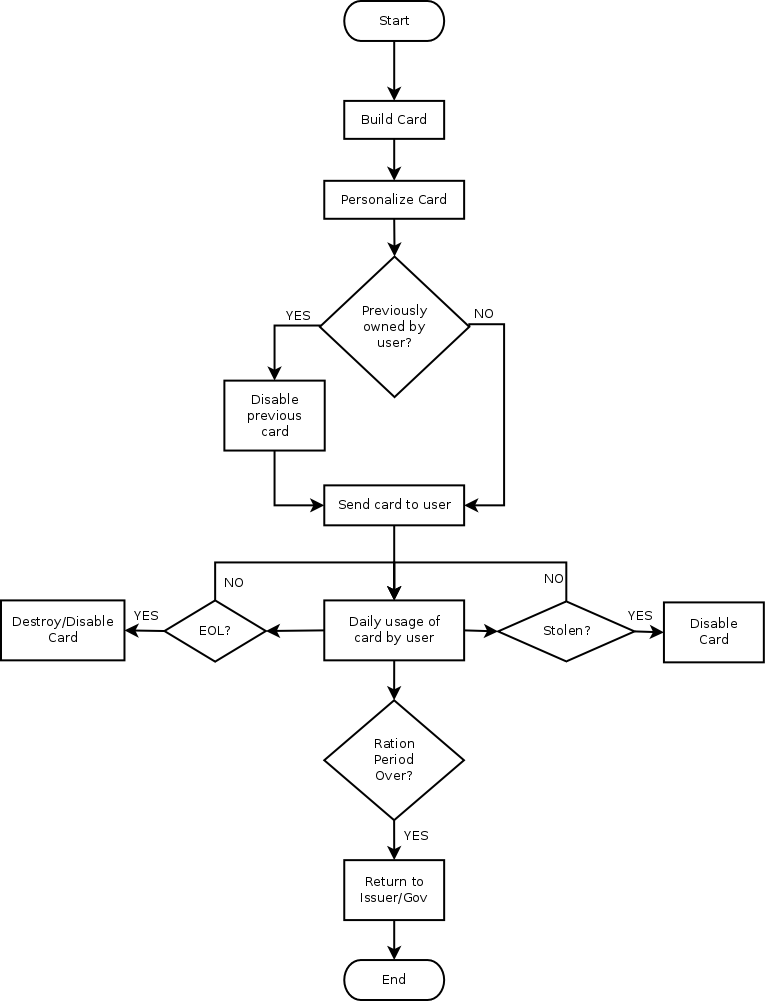
\includegraphics[width=\textwidth]{SCLifeCycle}

\subsection{Protocol Descriptions}

\subsubsection{Terminology}
    \begin{center}
        \begin{tabular}{| l | p{8cm} |}
            \hline
            $ENC\{X\}$ & encryption function for X with symmetric key agreed to by both parties\\ \hline
            $SIG\{X\}_{privkey}$ & signing function for X with private key of sender \\ \hline
            $[X]_{pubkey}$ & encryption function for X with a public key of the sender \\ \hline
            $certificate_{T}$ & certificate of Terminal \\ \hline
            $pub_{T}$ & public key of Terminal \\ \hline
            $priv_{T}$ & private key of Terminal  \\ \hline
            $ID_{T}$ & Identification (ID) number of Terminal \\ \hline
            $SK$ & Symmetric Key \\ \hline
            $Verify$ & Certificate Verification function \\ \hline
            $Log$ & Logging function to keep track of transactions \\ \hline
            $T$ & Terminal (charging/petrol) \\ \hline
            $PC$ & Petrol Card \\ \hline
            $BE$ & Back-end \\ \hline
            $VTS$ & Valid timestamp until certificates are considered untrusted (24Hours from the time the CVR was requested) \\ \hline
            $TS$ & Timestamp \\ \hline
            $Certs$ & List of certificates that are valid and or revoked \\ \hline
            $CVR$ & Certificate Validity Request function \\ \hline
            $PIN$ & PIN number \\ \hline
            $PIN_{AUTH}$ & Boolean response to indicate validity of PIN \\ \hline
            $Calc$ & Petrol points calculation function based on current balance \& pumped amount (in liters) \\ \hline
            $B$ & current petrol points (in liters) \\ \hline
            $UB$ & used up petrol points (in liters) \\ \hline
        \end{tabular}
    \end{center}

\subsubsection{Mutual Authentication}
First the terminal sends a command APDU to enable the correct applet from the petrol card for the petrol rationing system. After that the terminal sends its certificate and public key to the petrol card. The petrol card verifies the certificate of the terminal and chooses a symmetric key for encrypted communication. The petrol card signs its identification number with its private key, encrypts that signature and its own certificate with the symmertric key. Then it sends the encrypted signature and certificate together with the symmetric key encrypted by the public key of the terminal. Once the terminal receives the certificate of the petrol card, it verifies it. It then sends signs its won signature with its private key and then combied with a signed version of the identification, encrypts them both with the symmetric key and sends it to the petrol card.
\\

T $\to$ PC: commandAPDU to enable applet.\\
T $\to$ PC: $certificate_{T}, pub_{T}$\\
PC: $Verify(certificate_{T})$ and choose SK\\
PC $\to$ T: $ENC\{SIG\{ID_{PC}\}_{priv_{PC}}, certificate_{PC}\},  [ENC]_{pub_T}$\\
T: $Verify(certificate_{PC})$\\
T $\to$ PC: $ENC\{SIG\{ID_{T}\}_{priv_T}, ID_{T}\}$ \\
and now we have a secure channel between a terminal and a petrol card.

\subsubsection{Certificate Validity Request}
After mutual authentication has been done, the petrol card will request the certificate revocation list from the back-end through the terminal. In this case, the terminal just acts as a relay between the petrol card and the back-end.
\\
\\
PC $\to$ BE: $[CVR + pub_{PC}]_{pub_{BE}}$\\
BE $\to$ PC: $[SIG\{VTS, TS, Certs\}_{priv_{BE}}, VTS, TS, Certs]_{pub_{PC}}$

\subsubsection{PIN validation and authentication of card owner}
After mutual authentication has been done, the terminal receives a PIN on the numpad from the card owner, signs the PIN and send the encryption of the signature with the plaintext PIN number to the petrol card. Once the petrol card receives the PIN number, returns the encrypted and signed boolean value (True/False) to the terminal after it verifies the PIN number.
\\
\\
PIN validation and authentication of card owner guarantees security requirment 1(d).
\\
\\
T $\to$ PC: $ENC\{SIG\{PIN\}_{priv_T}, PIN\}$\\
PC $\to$ T: $ENC\{SIG\{PIN_{AUTH}\}_{priv_{PC}}, PIN_{AUTH}\}$

\subsubsection{Getting petrol from the petrol terminal}
After mutual authentication, PIN validation and authentication of card owner has been done, the petrol card can send its current balance to the petrol terminal for getting petrol. Then, the terminal writes a balance of zero to the petrol card for cases where the card was removed mid transaction. Once the petrol has been pumped and the user successfully terminates the program, the terminal writes a new balance after deducting the pumped petrol amount from the initial balance sent by the card, to the card. And immediately after that the terminal logs the time, identification number, balance and the amount of petrol pumped by the user.
\\
\\
PC $\to$ T: $ENC\{SIG\{B\}_{priv_{PC}}, B\}$\\
T $\to$ PC: $ENC\{SIG\{BZ\}_{priv_T}, BZ\}$\\
T: $Calc\{B = B - UB\}$\\
T $\to$ PC: $ENC\{SIG\{B\}_{priv_T}, B\}$\\
T: $LOG\{TS, ID_{PC}, B, UB\}$

\subsubsection{Charging petrol allowance to the petrol card}
After mutual authentication, PIN validation and authentication of card owner
has been done, the petrol card can ask the charging terminal to charge its
allowed monthly petrol balance. Then the terminal starts a secure channel
between itself and the back-end to get the monthly petrol allowance, and then
writes those values back to the petrol card.
\\
\\
The terminal starting a secure channel with the back-end to get the monthly petrol allowance guarantees security requirement 1(e) \& 3(c).
\\
\\
PC $\to$ T: requestAPDU to initiate charging monthly allowance \\
T: creates secure channel and requests monthly allowance from back-end \\
T $\to$ PC: $ENC\{SIG\{B,TS\}_{priv_{BE}}, B, TS\}$
